\subsection{Állapotok}

\subsubsection{Első iteráció - 2019.10.14}

\tab \textit{Ebben a fázisban még nem volt meg a megfelelő tudás a véges állapotú adatútas automatáról.
Itt a tervezés elnagyolva volt elvégezve, még nem volt kellőképpen átlátva a megoldandó probléma. A négy kontrolljel közül (start, reset, clear, stop)
csak kettő lett végül felhasználva: start és reset.}

Állapotok:
\begin{itemize}
\item READY
	\begin{itemize}
	\item Alap állapot 
	\item "reset" jel esetén ide kerül vissza az automata
	\end{itemize}
\item INIT
	\begin{itemize}
	\item minden LED-et kikapcsol (0x000000-t ír)
	\item "clear" jel esetén ide kerül az automata
	\end{itemize}
\item RENDER
	\begin{itemize}
	\item egyenként küldi a szín információt a LED-ekre
	\item annyiszor végződik el itt a művelet, ahány LED-ünk van
	\item "stop" jel esetén megáll a kiírás
	\end{itemize}
\item DISPLAY
	\item megtörtént a kiírás
\end{itemize}

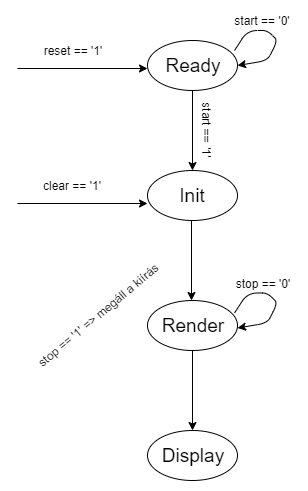
\includegraphics[scale=0.5]{allapotdiagram.png}

\subsubsection{Második iteráció - 2019.10.28}

\tab \textit{Ebben a fázisban kezdett kialakulni a szükséges tudás a feladat megoldásához, és a feladat is már jobban át volt látva. Itt már egy nagy modul helyett, két kisebb modulra van kigondolva
a feladat megoldása.}

\tab Állapotdiagram átírva úgy, hogy a küldési logikát is tartalmazza:

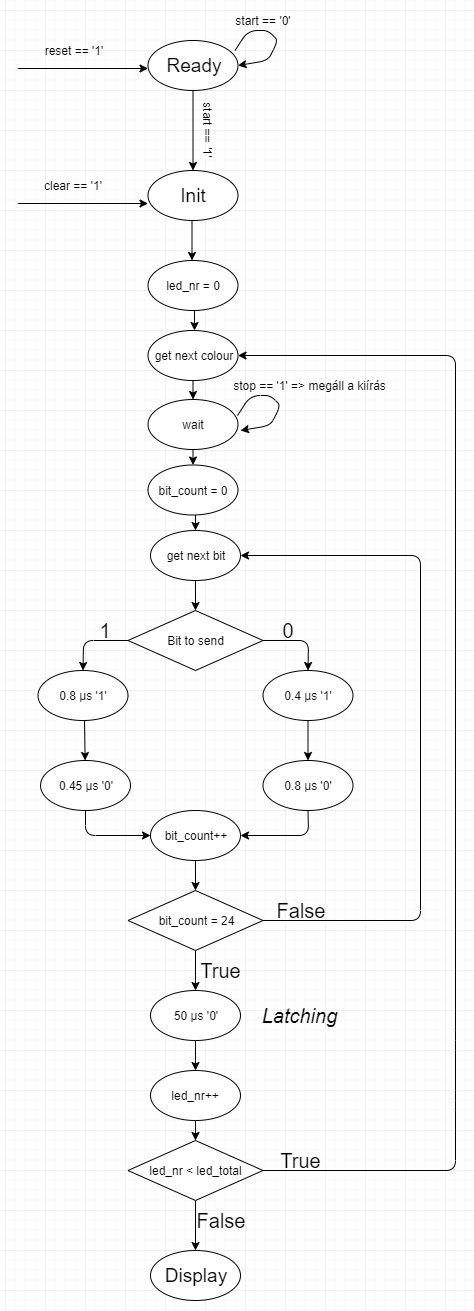
\includegraphics[scale=0.4]{allapotdiagram_2.png}

\tab \textit{Egy kisebb finomítás az állapotdiagramon. Itt már le van bontva részletesen az diagram RT műveletekre.}

\tab Állapotdiagram egy 90 LED-et vezérlő modulra

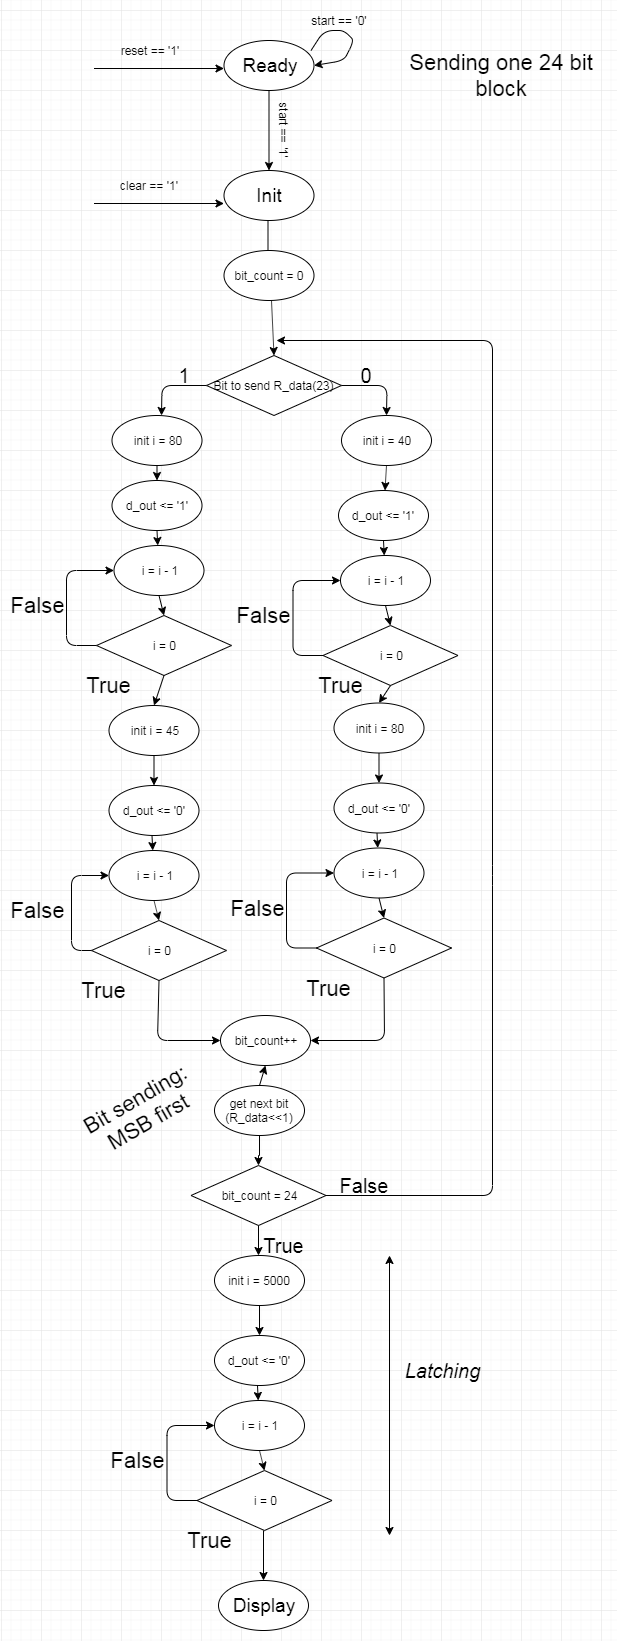
\includegraphics[scale=0.4]{allapotdiagram_3.png}


\subsection{Alegységek}

\subsubsection{Első iteráció - 2019.10.14}

\begin{itemize}
\item Következő állapot regiszter \textbf{\textit{Next State Register}}
\item Állapot regiszter \textbf{\textit{State Register}}
\item Szín regiszter \textbf{\textit{Colour Register}}
\item Küldési logika regiszter \textbf{\textit{Transmission Logic Register}}
\end{itemize}

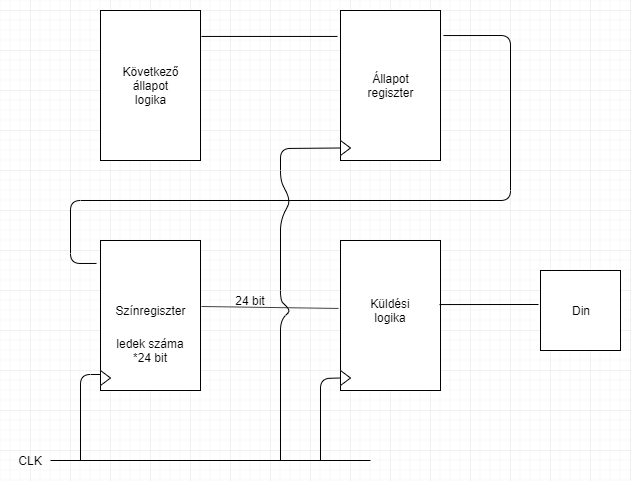
\includegraphics[scale=0.5]{tombvazlat.png}

\tab \textbf{Küldési logika regiszter}

\noindent A küldési logika modul részletesebb lebontása: 

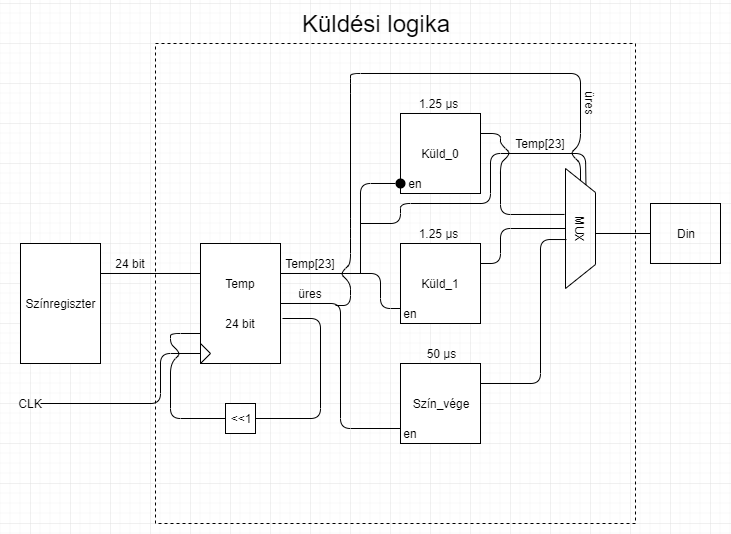
\includegraphics[scale=0.6]{kuldesi_logika.png}

\subsubsection{Második iteráció - 2019.10.28}

\tab Minden \textbf{led\_controll} modulhoz tartozik egy BRAM blokk és minden ilyen modul egy ledfűzért vezérel meg. Öt ilyen blokk megvezérel öt ledfűzért, ezáltal létrehozva a ledmátrixot.
Az órajel, start, reset, stop és data-rd jelek közösek minden modulnak.

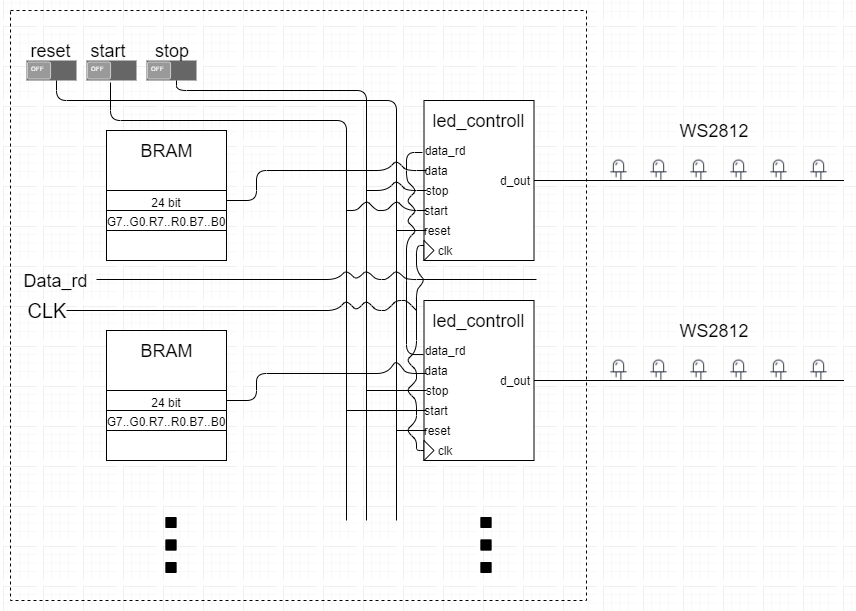
\includegraphics[scale=0.5]{tombvazlat2.png}


\subsection{Idődiagram}

\subsubsection{Első iteráció - 2019.10.26}

\tab \textit{Ebben a fázisban az volt az elgondolás, hogy a modul akkor olvassa be az adatot a \textbf{data} sínről, ha a \textbf{data\_rd} jel 1-es. Mint később kiderült,
erre nincs szükség.}

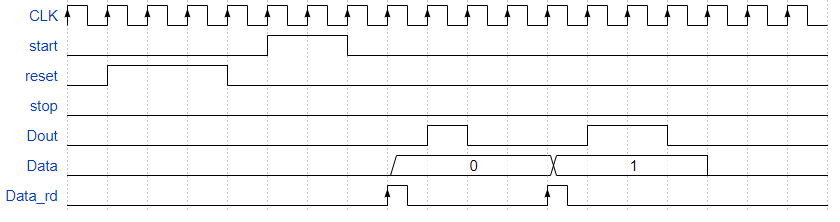
\includegraphics[scale=0.6]{general.PNG}

\begin{itemize}
\item CLK: 100 MHz-es órajel
\item start: jel a folyamat elindításához
\item reset: jel a folyamat resetálásához
\item stop: jel a kiírás megállításához. Csak két 24 bit-es blokk kiírása közben tudja megállítani a kiírást
\item Dout: Egyszálú adatsín a LED-ekre.
\item Data: Kiírandó adat, Data\_rd felmenő órajelére olvassa be az adatot.
\item Data\_rd: Aktiváló bit az adat beolvasására
\end{itemize}